\chapter{Experimental results\label{sec:experimentalresults}}

In this chapter I describe the design of the experiments made to load test the Signal server architectures and I report the obtained results.

\section{Metrics\label{sec:metrics}}

The metrics considered the response times of the system under load tests.

To make the implemented tests usable in a black box way, avoiding any kind of knowledge regarding the internal operations of the server, I only used the APIs offered by the server itself.

The metrics used for the requests are the following ones:
\begin{itemize}
    \item average response time per request type;
    \item median response time per request type;
    \item 90th, 95th and 99th percentile response time per request type.
\end{itemize}

The metrics used to measure the server load are the following ones:
\begin{itemize}
    \item percentage of memory used per second;
    \item percentage of CPU used per second;
    \item network I/O (B/s).
\end{itemize}

With these metrics it is possible to verify which requests require more time to get a response and which ones have a higher impact on the server load.

It is possible to know which are the most used components of the architecture and which requests are a weak point for the system by understanding the interactions among them.



\section{Environment characteristics\label{sec:environment}}

Here there are some details for the reproducibility of the experiments, so a technical description of the server used and of the client used on them.

\subsection{Server characteristics\label{sec:servercharacteristics}}

The server side used to run the experiments is a fully scaled reproduction of the Signal server from their source code, apart from some components, for example the one used in production from Signal in order to make possible an encrypted contact discovery at hardware level \cite{signal_cds}.

The deployment of the server side has been done on the AWS infrastructure, because it is used on the most recent version of the Signal server and on less recent version for some provided services, such as AWS SQS\footnote{\url{https://aws.amazon.com/sqs}} and DynamoDB.

I deployed the server to a t3.micro EC2 instance\footnote{\url{https://aws.amazon.com/ec2/instance-types}}, which is included in the free resources plan of AWS.
It provides:
\begin{itemize}
    \item $2$ vCPUs of burstable type;
    \item $1$ GB of RAM;
    \item $30$ GB of SSD.
\end{itemize}

The software level characteristics are listed here:
\begin{itemize}
    \item OS: Ubuntu 20.04.3 LTS\footnote{\url{https://ubuntu.com}}
    \item Dropwizard 2.0.13 (Signal 4.97) / 2.0.22 (Signal 6.13)
    \item Redis server v=5.0.7
    \item PostgreSQL 12.9
    \item Nginx 1.18.0\footnote{\url{https://www.nginx.com}}
\end{itemize}

In order to make it reachable from the outside I used ClouDNS\footnote{\url{https://www.cloudns.net}}, which provides a free dynamic DNS for subdomains. The name I chose is \url{signal.cloudns.cc}

\subsection{Client characteristics\label{sec:clientcharacteristics}}

In order to perform the test it has been used JMeter \cite{apache_jmeter}, a general purpose tool used for load testing analysis.
To perform the tests I used my laptop, which was enough for the characteristics of the server side.

The resources of the laptop are the following:
\begin{itemize}
    \item Intel(R) Core(TM) i3-4005U CPU @ $1.70$GHz;
    \item $4$GB of DDR3 RAM;
    \item $500$GB of SSD.
\end{itemize}

The software level characteristics are listed here:
\begin{itemize}
    \item OS: Ubuntu 21.04
    \item Apache JMeter 5.4.1
\end{itemize}

\section{Details about implementation\label{sec:implementation}}

To implement the load experiments I used JMeter, a Java tool made to generate a huge number of requests with lots of parameters.

\subsection{Base load settings\label{sec:baseloadsettings}}

With base load we mean a low load with a long duration, used to simulate the use of Signal without particular events.

The base load is very low also because of the server capacity. The test is made from one user who executes a sequence of operations for account creations or to send messages. It is executed one sequence at a time, for $1000$ consecutive times.

Here I report the settings used to generate a base load for a long period of time on the server using JMeter.

\begin{figure}[H]
    \centering
    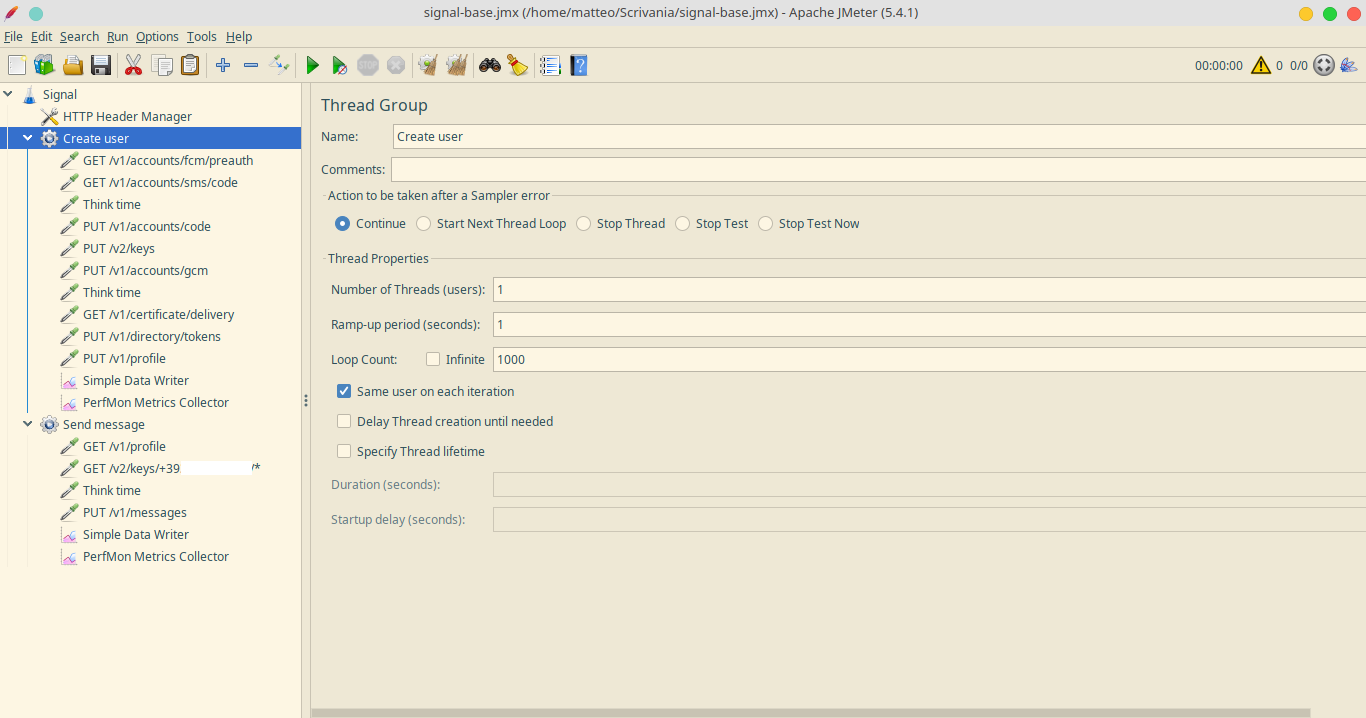
\includegraphics[width=\textwidth]{images/signal-create-base}
    \caption{JMeter base load for accounts creation}
    \label{fig:jmeterbaseuser}
\end{figure}

As the figure shows, the test performs $1000$ user creation, with $1$ thread at a time (so the ramp-up period is not used). So in total JMeter performs $8000$ calls to the server.

The same thing is done for the message sending base load, as the following figure shows.

\begin{figure}[H]
    \centering
    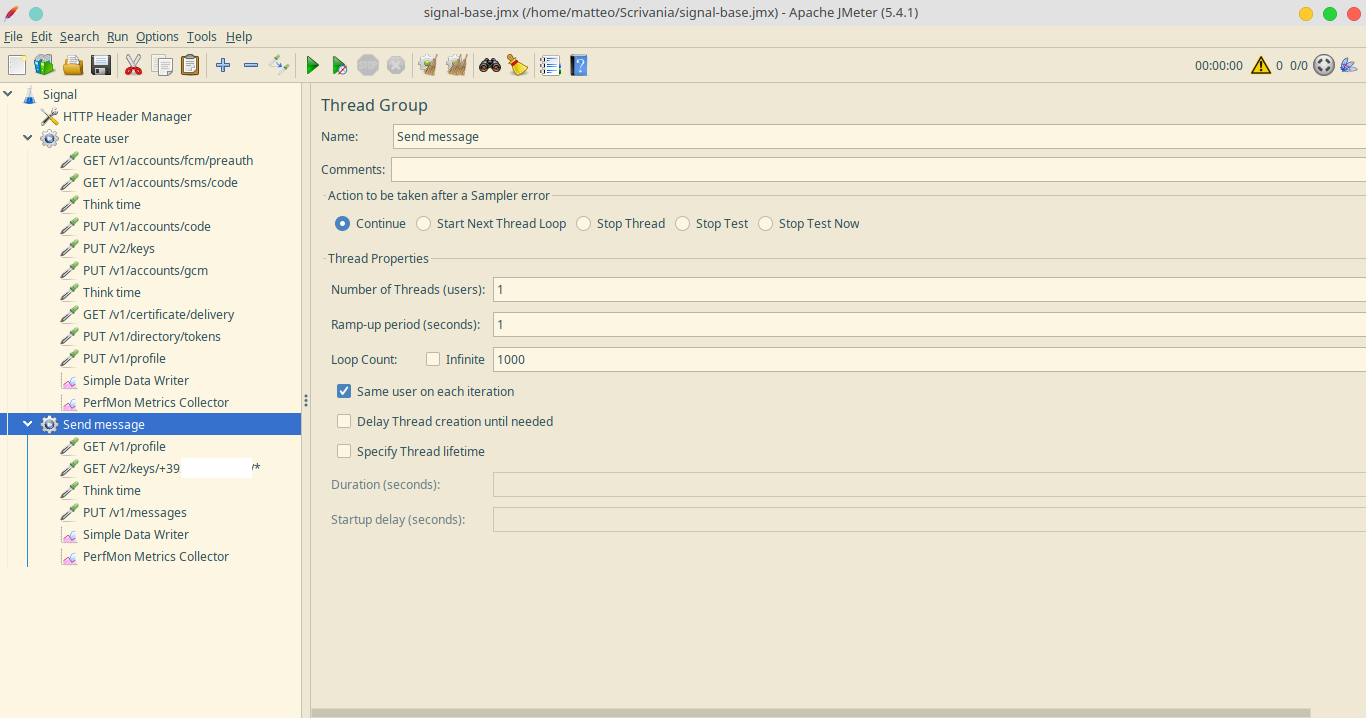
\includegraphics[width=\textwidth]{images/signal-message-base}
    \caption{JMeter base load for message sending}
    \label{fig:jmeterbasemessage}
\end{figure}

\subsection{High load settings\label{sec:highloadsettings}}

With high load we mean a load higher than the base one, with a low duration, used to simulate a higher use of the Signal applications. An example can be the New Year's Eve, where a lot of messages are sent in a specific period of time.



The load is high enough for the server because of the low capacity.
There is a limit of $100$ parallel users, who execute sequences of requests to the Signal APIs to create accounts or to send messages. Each user is added after $2$ seconds (ramp-up of $200$ seconds) and the experiment is repeated $10$ times.

In order to perform a higher load test, for a shorter period of time, I used the following settings.

\begin{figure}[H]
    \centering
    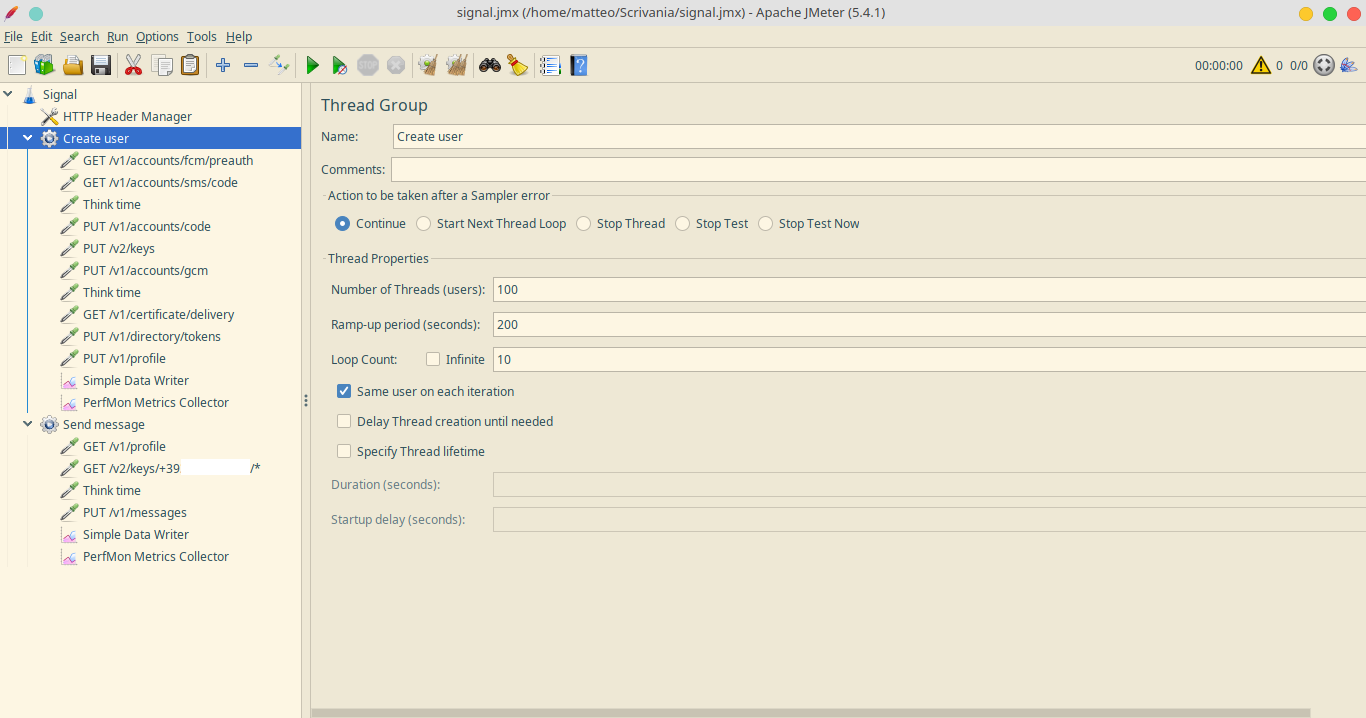
\includegraphics[width=\textwidth]{images/signal-load}
    \caption{JMeter high load test}
    \label{fig:jmeterhighload}
\end{figure}

This time the maximum concurrent threads is set to $100$, with a ramp-up period of $200$ seconds (a thread is added every $2$ seconds), with $10$ cycles.
This means that the users created are still $1000$.

\begin{figure}[H]
    \centering
    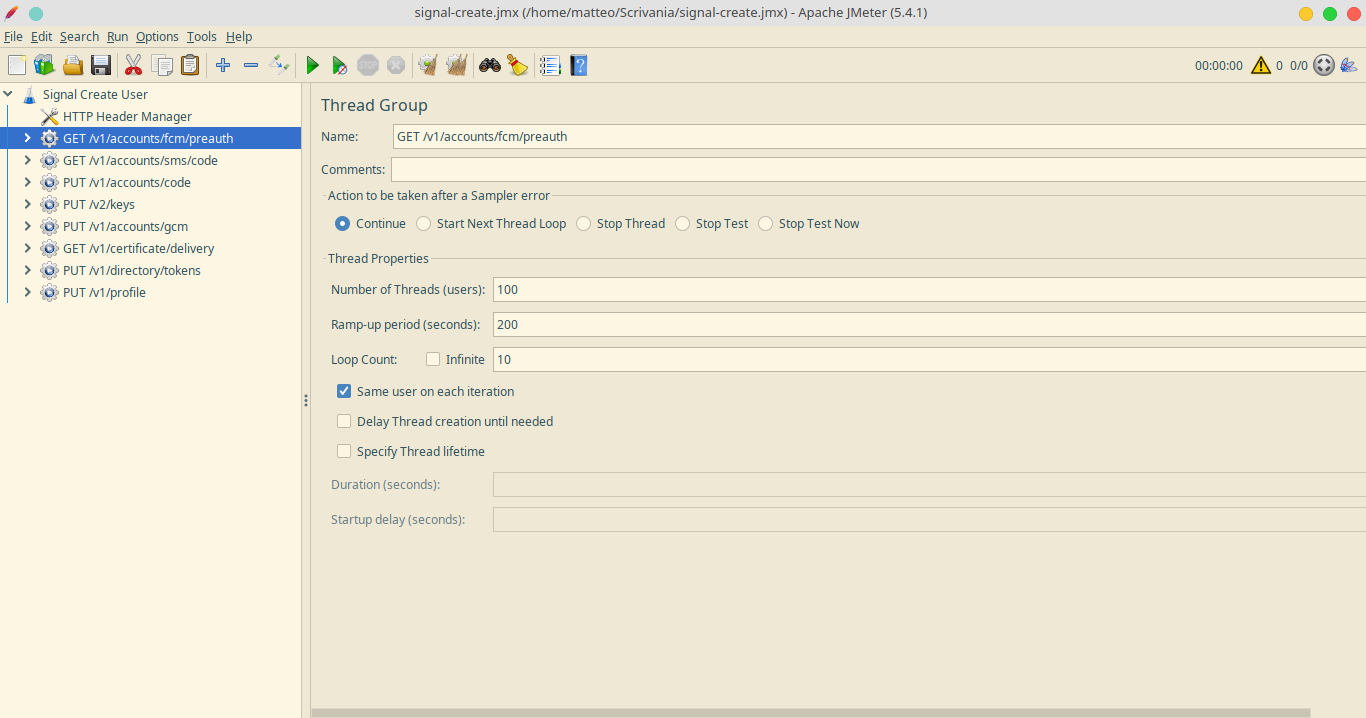
\includegraphics[width=\textwidth]{images/signal-create-load}
    \caption{JMeter high load for accounts creation}
    \label{fig:jmeterhighloadcreate}
\end{figure}

The same thing has been done for the message sending, and also for the single requests divided by type.

\begin{figure}[H]
    \centering
    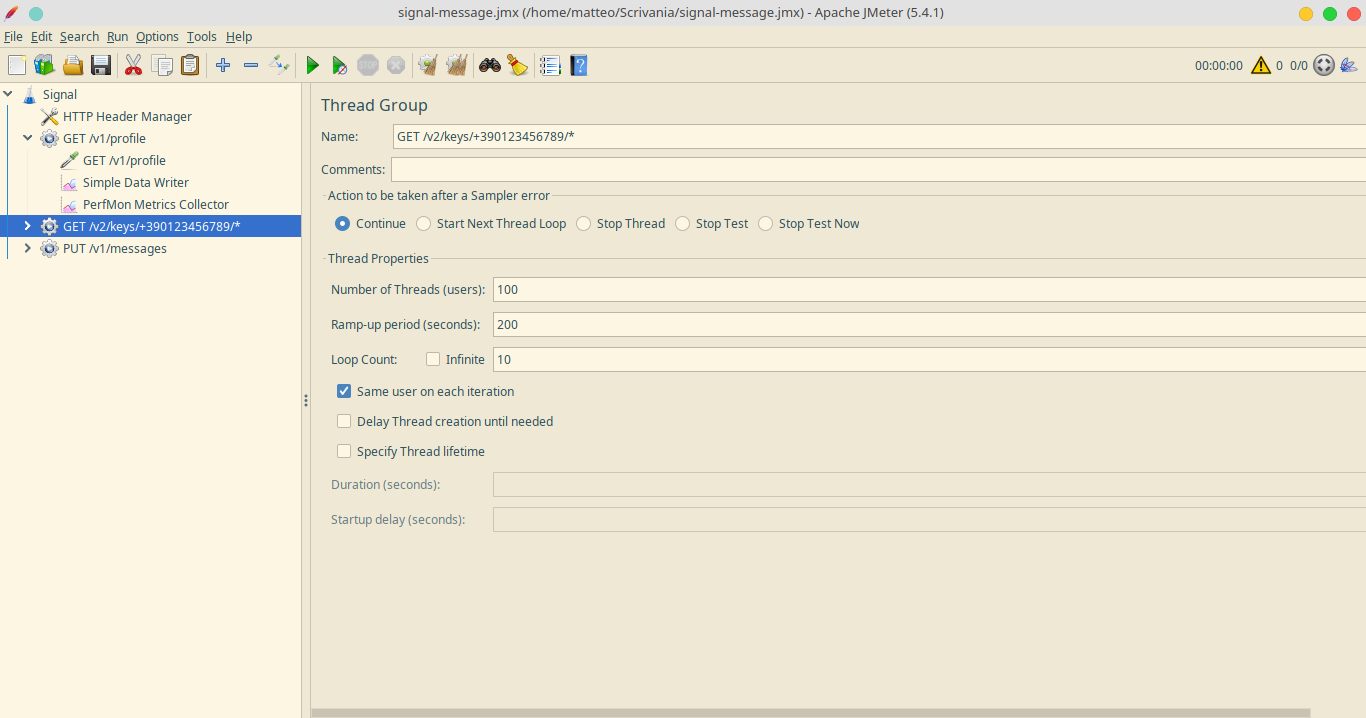
\includegraphics[width=\textwidth]{images/signal-message-load}
    \caption{JMeter high load for message sending}
    \label{fig:jmeterhighloadmessage}
\end{figure}

\subsection{Perfmon\label{sec:perfmon}}

Perfmon\footnote{\url{https://jmeter-plugins.org/wiki/PerfMon}} is a plugin made for JMeter which is used to collect metrics about the resources of the machine which is tested.
I used it to collect data about the CPU usage, the RAM usage and the network performance during the tests.

\begin{figure}[H]
    \centering
    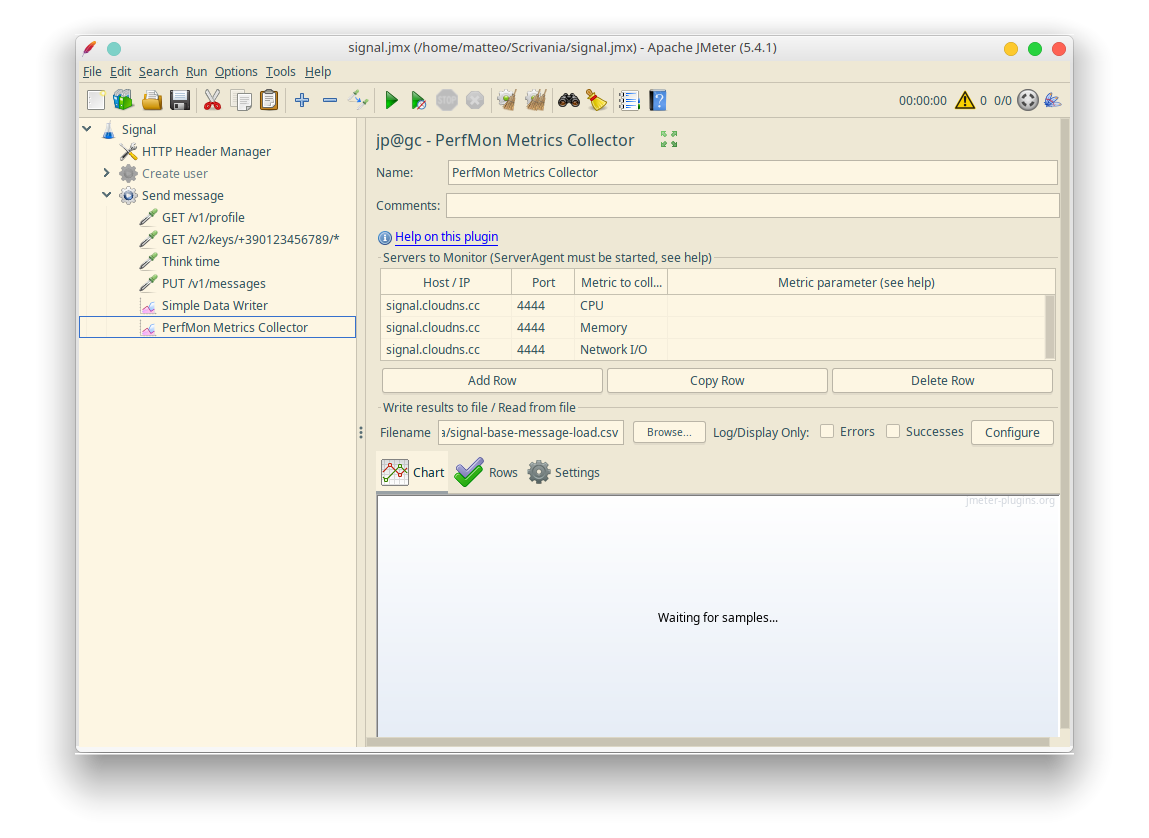
\includegraphics[width=\textwidth]{images/perfmon}
    \caption{JMeter Perfmon plugin}
    \label{fig:jmeterperfmon}
\end{figure}



\section{Results\label{sec:results}}

In this section I report the measures found by the test executions on both of the server versions, and some observations on them.

\subsection{New user registration\label{sec:newuser}}

All the Signal APIs are managed by the Dropwizard controllers, the framework used in order to implement the server orchestrator.

The experiment uses the following calls to the REST APIs of the Signal server:

\begin{table}[H]
\resizebox{\textwidth}{!}{%
\begin{tabular}{llll}
\hline
\multicolumn{1}{c}{\textbf{Type of request}} & \multicolumn{1}{c}{\textbf{Request path}} & \multicolumn{1}{c}{\textbf{Description}} & \multicolumn{1}{c}{\textbf{Involved components}} \\ \hline
GET & /v1/accounts/fcm/preauth & Request a preauth to Firebase Cloud Message & Dropwizard, Redis, PostgreSQL/DynamoDB, GCM \\
GET & /v1/accounts/sms/code & Request an OTP code, sent using Twilio & Dropwizard, Redis, PostgreSQL/DynamoDB, GCM, Twilio \\
PUT & /v1/accounts/code & Send the received code from Twilio & Dropwizard, Redis, PostgreSQL/DynamoDB, AWS SQS \\
PUT & /v2/keys & Send the keys for encryption protocol & Dropwizard, Redis, PostgreSQL/DynamoDB \\
PUT & /v1/accounts/gcm & Send details for Google Cloud Message & Dropwizard, Redis, PostgreSQL/DynamoDB, AWS SQS \\
GET & /v1/certificate/delivery & Get certificate from the Signal server & Dropwizard, Redis, PostgreSQL/DynamoDB \\
PUT & /v1/directory/tokens & Put tokens of Signal account & Dropwizard \\
PUT & /v1/profile & Put information of Signal account & Dropwizard,Redis, PostgreSQL/DynamoDB \\ \hline
\end{tabular}%
}
\caption{Sequence of calls to register a new account}
\label{tab:apiregistration}
\end{table}

Between the request for the Twilio OTP code and its insertion and between the insertion of the GCM data and the insertion of the profile data there are two intervals of 3 seconds to simulate the user time to do an action with precompiled fields.

\subsubsection{Base load for a long period of time on Signal 4.97}

Here there is a table with the measures obtained from the accounts' creation on Signal 4.97.

\begin{table}[H]
\resizebox{\textwidth}{!}{%
\begin{tabular}{@{}lllllllllll@{}}
\toprule
\multicolumn{1}{c}{\multirow{2}{*}{\textbf{Request}}} & \multicolumn{1}{c}{\multirow{2}{*}{\textbf{\#Samples}}} & \multicolumn{7}{c}{\textbf{Response times (ms)}} & \multicolumn{2}{c}{\textbf{Network (KB/s)}} \\ \cmidrule(l){3-11} 
\multicolumn{1}{c}{} & \multicolumn{1}{c}{} & \multicolumn{1}{c}{Average} & \multicolumn{1}{c}{Min} & \multicolumn{1}{c}{Max} & \multicolumn{1}{c}{Median} & \multicolumn{1}{c}{90th pct} & \multicolumn{1}{c}{95th pct} & \multicolumn{1}{c}{99th pct} & \multicolumn{1}{c}{Received} & \multicolumn{1}{c}{Sent} \\ \midrule
GET /v1/accounts/fcm/preauth & 1000 & 37.91 & 20 & 744 & 28.00 & 36.00 & 52.95 & 288.98 & 0.07 & 0.07 \\
GET /v1/accounts/sms/code & 1000 & 35.46 & 19 & 552 & 26.00 & 35.90 & 51.00 & 290.92 & 0.15 & 0.05 \\
GET /v1/certificate/delivery & 1000 & 44.72 & 19 & 2261 & 27.00 & 59.90 & 107.00 & 312.96 & 0.14 & 0.05 \\
PUT /v1/accounts/code & 1000 & 44.64 & 20 & 1113 & 27.00 & 54.00 & 123.40 & 342.90 & 0.08 & 0.09 \\
PUT /v1/accounts/gcm & 1000 & 37.39 & 18 & 590 & 27.00 & 35.00 & 55.85 & 296.81 & 0.07 & 0.08 \\
PUT /v1/directory/tokens & 1000 & 57.44 & 41 & 1236 & 47.00 & 54.00 & 67.00 & 322.90 & 0.07 & 0.49 \\
PUT /v1/profile & 1000 & 43.46 & 24 & 551 & 34.00 & 48.90 & 61.95 & 277.99 & 0.07 & 0.10 \\
PUT /v2/keys & 1000 & 70.72 & 50 & 660 & 59.00 & 70.00 & 90.85 & 351.93 & 0.07 & 0.66 \\ \bottomrule
\end{tabular}%
}
\caption{Base load accounts' creation on Signal 4.97}
\label{tab:baseloadregisterold}
\end{table}

From these data we can see that the calls used to save the keys request an higher time compared to the other requests.
This delay is due to the higher weight of the message, which contains a lot of keys, so it is heavier compared to the other messages.

All the requests which require read/write operations on a database involve Redis, which can trigger requests to PostgreSQL.
This is useful, Redis act as a database in RAM, so it is more efficient compared to PostgreSQL.

If we order the requests by the average response time we see that the weak point is always the dimension of the request instead of the component used in the architecture.

\begin{figure}[H]
    \centering
    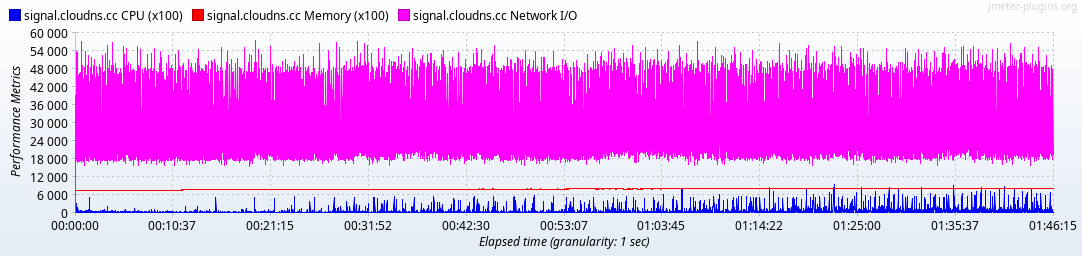
\includegraphics[width=\textwidth]{images/497/signal-base-create-load}
    \caption{Base load accounts' creation on Signal 4.97}
    \label{fig:signalbasecreateloadold}
\end{figure}

From the diagram it is visible that the CPU use increase over time, also if their number is low and there are pauses between the requests.
The diagram shows also that the CPU use is not constant and that it goes from $0$\% to $100$\% and vice versa alternatively.

\subsubsection{High load with ramp-up on Signal 4.97}

Here I show the data obtained from the high load generation with a ramp-up for the accounts' creation.

\begin{table}[H]
\resizebox{\textwidth}{!}{%
\begin{tabular}{@{}lllllllllll@{}}
\toprule
\multicolumn{1}{c}{\multirow{2}{*}{\textbf{Request}}} & \multicolumn{1}{c}{\multirow{2}{*}{\textbf{\#Samples}}} & \multicolumn{7}{c}{\textbf{Response times (ms)}} & \multicolumn{2}{c}{\textbf{Network (KB/s)}} \\ \cmidrule(l){3-11} 
\multicolumn{1}{c}{} & \multicolumn{1}{c}{} & \multicolumn{1}{c}{Average} & \multicolumn{1}{c}{Min} & \multicolumn{1}{c}{Max} & \multicolumn{1}{c}{Median} & \multicolumn{1}{c}{90th pct} & \multicolumn{1}{c}{95th pct} & \multicolumn{1}{c}{99th pct} & \multicolumn{1}{c}{Received} & \multicolumn{1}{c}{Sent} \\ \midrule
GET /v1/accounts/fcm/preauth & 953 & 177.24 & 20 & 57250 & 37.00 & 106.00 & 147.30 & 455.64 & 1.46 & 1.36 \\
GET /v1/accounts/sms/code & 951 & 104.41 & 18 & 43321 & 27.00 & 66.00 & 81.00 & 193.60 & 3.16 & 0.92 \\
GET /v1/certificate/delivery & 946 & 87.58 & 18 & 5534 & 26.50 & 70.30 & 102.60 & 2509.52 & 3.54 & 1.17 \\
PUT /v1/accounts/code & 950 & 122.05 & 18 & 22948 & 27.00 & 87.00 & 119.45 & 1503.15 & 1.92 & 2.02 \\
PUT /v1/accounts/gcm & 946 & 66.39 & 19 & 5541 & 26.00 & 62.00 & 89.65 & 378.28 & 1.79 & 2.00 \\
PUT /v1/directory/tokens & 946 & 135.69 & 41 & 12532 & 48.00 & 94.30 & 126.95 & 3836.24 & 1.77 & 11.81 \\
PUT /v1/profile & 946 & 1054.17 & 24 & 80726 & 41.00 & 105.60 & 178.90 & 69366.33 & 1.48 & 1.93 \\
PUT /v2/keys & 950 & 310.79 & 51 & 58985 & 71.00 & 109.00 & 133.00 & 1727.85 & 1.38 & 12.78 \\ \bottomrule
\end{tabular}%
}
\caption{High load accounts' creation on Signal 4.97}
\label{tab:highloadregisterold}
\end{table}



The 99th percentile shows very high response times, because some requests, in order to be included in the curve, raise the maximum level of the percentile. They are next to the break point, which happened near the end of the experiment run.

\begin{figure}[H]
    \centering
    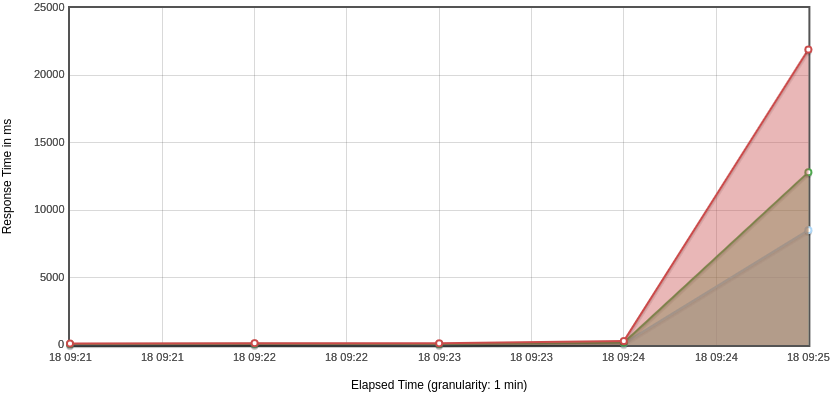
\includegraphics[width=\textwidth]{images/497/highloadregisteroldpct}
    \caption{Percentiles of high load accounts' creation on Signal 4.97}
    \label{fig:signalbasecreateloadoldpct}
\end{figure}

Also in this experiment the requests that required more time are the ones with the heavier message body, excluded the ones which are close to the break point.

\begin{figure}[H]
    \centering
    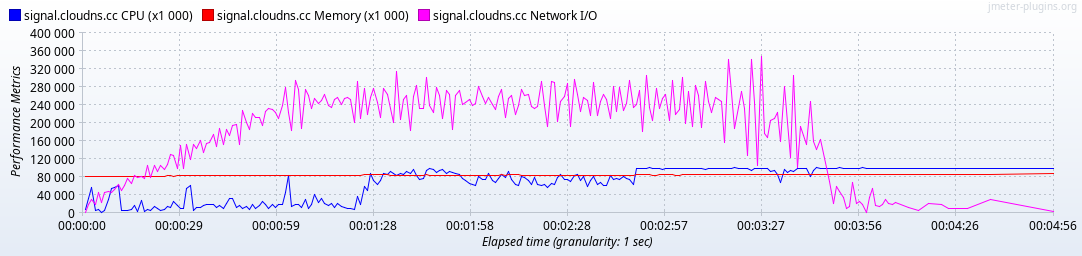
\includegraphics[width=\textwidth]{images/497/signal-create-load}
    \caption{High load accounts' creation on Signal 4.97}
    \label{fig:signalcreateloadold}
\end{figure}

The diagram shows that the server started to run at $100$\% of CPU load after $3$ minutes from the start of the experiment run, and it reached the break point at $3$ minutes and $40$ seconds, when the requests are not taken into account anymore.

To check which requests require more resources I do again the same experiment by request type.

\begin{figure}[H]
    \centering
    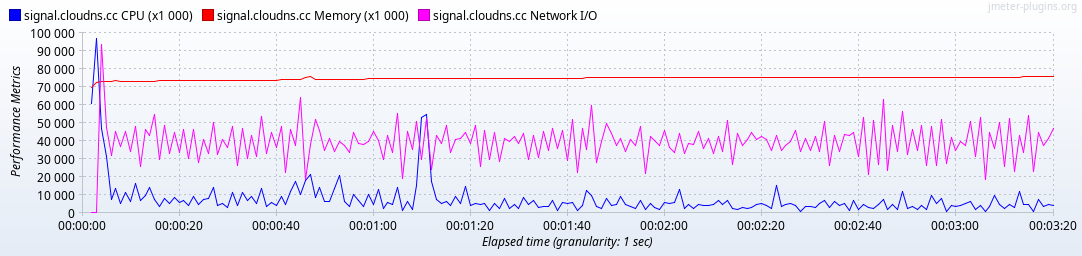
\includegraphics[width=\textwidth]{images/497/create-load-1}
    \caption{High load GET /v1/accounts/fcm/preauth on Signal 4.97}
    \label{fig:signalload1old}
\end{figure}


\begin{figure}[H]
    \centering
    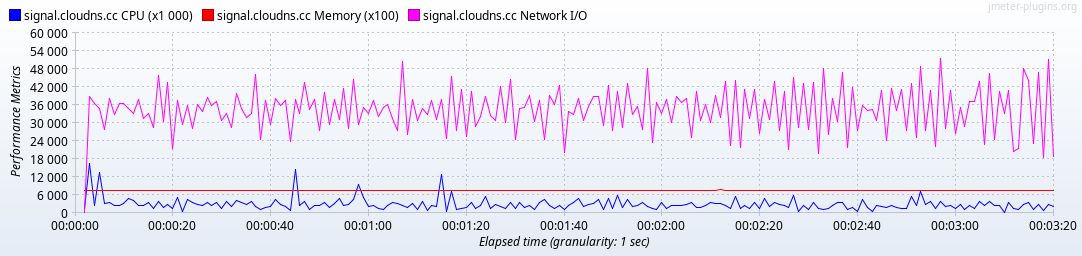
\includegraphics[width=\textwidth]{images/497/create-load-2}
    \caption{High load GET /v1/accounts/sms/code on Signal 4.97}
    \label{fig:signalload2old}
\end{figure}


\begin{figure}[H]
    \centering
    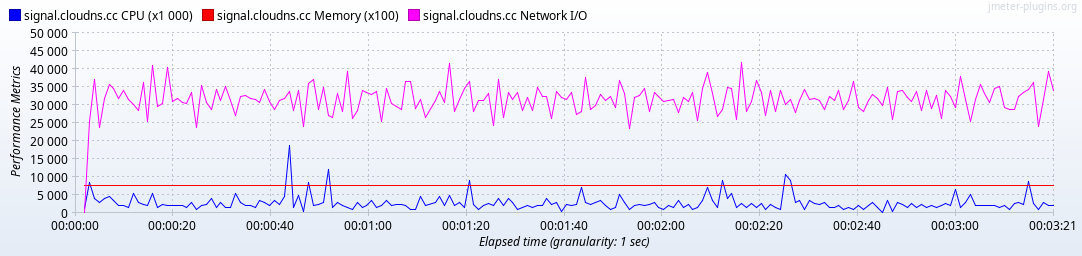
\includegraphics[width=\textwidth]{images/497/create-load-3}
    \caption{High load PUT /v1/accounts/code on Signal 4.97}
    \label{fig:signalload3old}
\end{figure}


\begin{figure}[H]
    \centering
    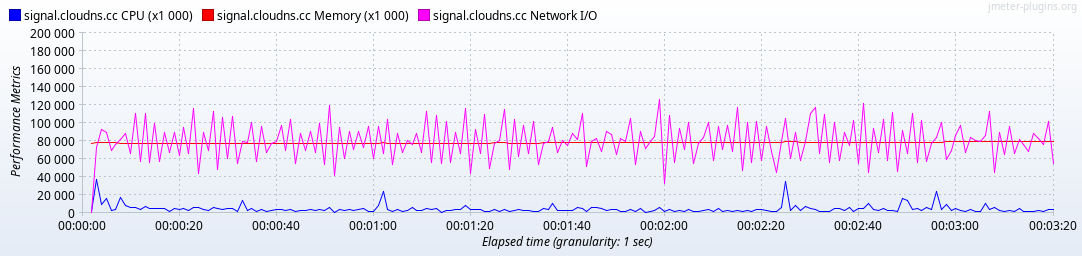
\includegraphics[width=\textwidth]{images/497/create-load-4}
    \caption{High load PUT /v2/keys on Signal 4.97}
    \label{fig:signalload4old}
\end{figure}


\begin{figure}[H]
    \centering
    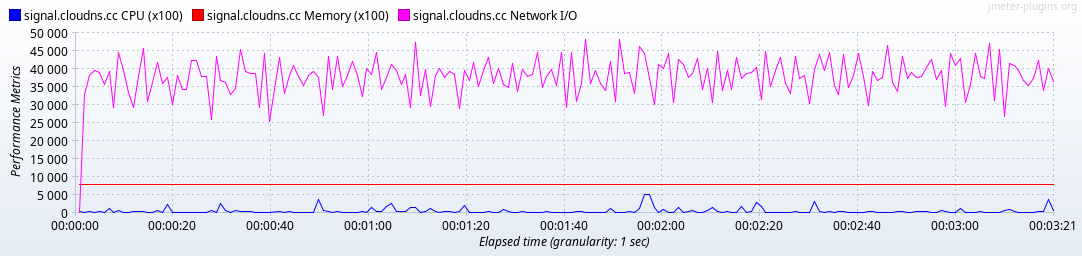
\includegraphics[width=\textwidth]{images/497/create-load-5}
    \caption{High load PUT /v1/accounts/gcm on Signal 4.97}
    \label{fig:signalload5old}
\end{figure}


\begin{figure}[H]
    \centering
    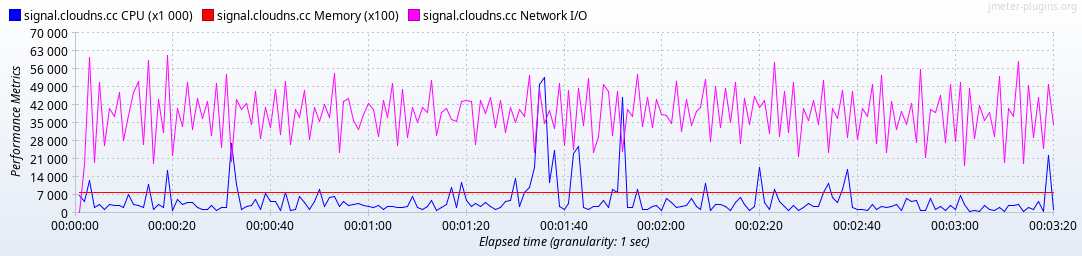
\includegraphics[width=\textwidth]{images/497/create-load-6}
    \caption{High load GET /v1/certificate/delivery on Signal 4.97}
    \label{fig:signalload6old}
\end{figure}


\begin{figure}[H]
    \centering
    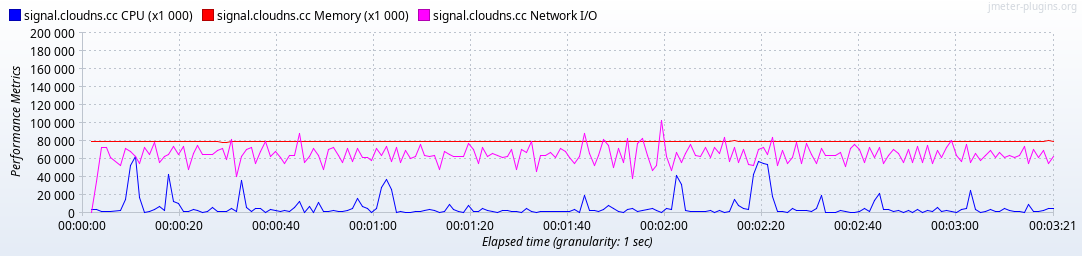
\includegraphics[width=\textwidth]{images/497/create-load-7}
    \caption{High load PUT /v1/directory/tokens on Signal 4.97}
    \label{fig:signalload7old}
\end{figure}


\begin{figure}[H]
    \centering
    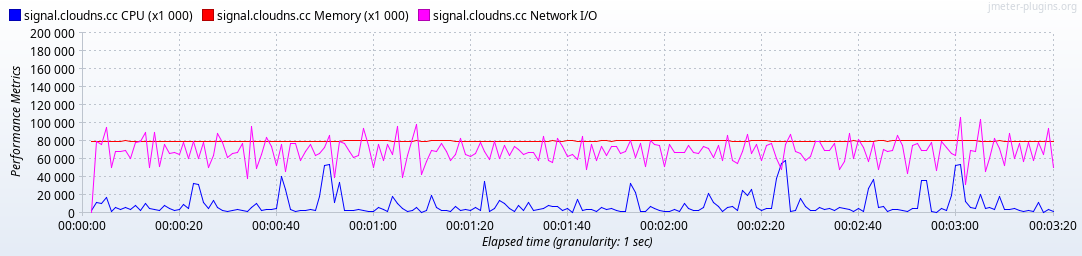
\includegraphics[width=\textwidth]{images/497/create-load-8}
    \caption{High load PUT /v1/profile on Signal 4.97}
    \label{fig:signalload8old}
\end{figure}

The obtained results confirm that all the requests are satisfied and no ramp-up happens.

So the overload of the first experiment is caused by the set of the requests, not from a particular one. None of the architectural components needs an excessive number of resources.

Now I compare the obtained results with the 6.13 server version.

\subsubsection{Base load for a long period of time on Signal 6.13}

Here I report the results for the accounts' creation on Signal 6.13.

\begin{table}[H]
\resizebox{\textwidth}{!}{%
\begin{tabular}{@{}lllllllllll@{}}
\toprule
\multicolumn{1}{c}{\multirow{2}{*}{\textbf{Request}}} & \multicolumn{1}{c}{\multirow{2}{*}{\textbf{\#Samples}}} & \multicolumn{7}{c}{\textbf{Response times (ms)}} & \multicolumn{2}{c}{\textbf{Network (KB/s)}} \\ \cmidrule(l){3-11} 
\multicolumn{1}{c}{} & \multicolumn{1}{c}{} & \multicolumn{1}{c}{Average} & \multicolumn{1}{c}{Min} & \multicolumn{1}{c}{Max} & \multicolumn{1}{c}{Median} & \multicolumn{1}{c}{90th pct} & \multicolumn{1}{c}{95th pct} & \multicolumn{1}{c}{99th pct} & \multicolumn{1}{c}{Received} & \multicolumn{1}{c}{Sent} \\ \midrule
GET /v1/accounts/fcm/preauth & 283 & 49.58 & 32 & 544 & 42.00 & 63.60 & 93.40 & 179.28 & 0.06 & 0.05 \\
GET /v1/accounts/sms/code & 283 & 36.87 & 20 & 171 & 30.00 & 47.00 & 89.60 & 154.16 & 0.12 & 0.04 \\
GET /v1/certificate/delivery & 282 & 310.26 & 21 & 73408 & 44.00 & 91.70 & 115.00 & 169.87 & 0.11 & 0.04 \\
PUT /v1/accounts/code & 282 & 48.27 & 21 & 363 & 40.00 & 76.70 & 100.85 & 318.17 & 0.07 & 0.07 \\
PUT /v1/accounts/gcm & 282 & 32.55 & 20 & 851 & 27.00 & 33.00 & 53.40 & 118.17 & 0.05 & 0.06 \\
PUT /v1/directory/tokens & 282 & 1177.65 & 41 & 317648 & 46.00 & 55.40 & 67.85 & 307.51 & 0.06 & 0.38 \\
PUT /v1/profile & 282 & 539.26 & 26 & 135067 & 54.50 & 96.00 & 119.55 & 200.68 & 0.07 & 0.08 \\
PUT /v2/keys & 282 & 70.45 & 52 & 415 & 65.00 & 86.00 & 100.00 & 164.99 & 0.05 & 0.51 \\ \bottomrule
\end{tabular}%
}
\caption{Base load accounts' creation on Signal 6.13}
\label{tab:baseloadregisternew}
\end{table}

The requests that show a higher response time are the one used to send the profile data and the one used to send the code, according to the 90th percentile and the 95th percentile.



We can see from the following diagram that the server is overloaded at the $30$th minute of execution, and the traffic gets stooped until an interruption.

\begin{figure}[H]
    \centering
    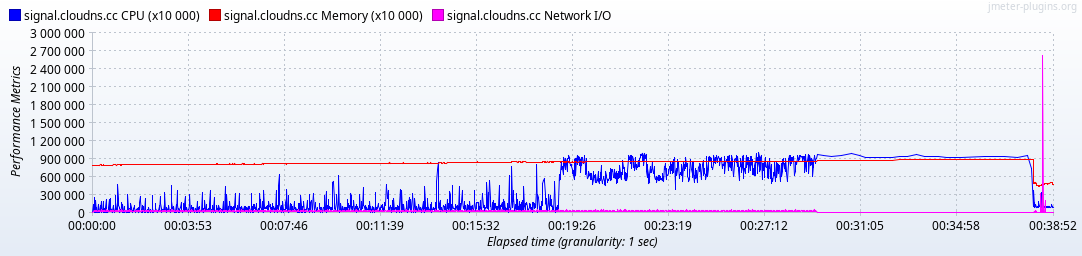
\includegraphics[width=\textwidth]{images/613/signal-base-create-load}
    \caption{Base load accounts' creation on Signal 6.13}
    \label{fig:signalbasecreateloadnew}
\end{figure}

This architecture, compared from the previous one, is more susceptible to a lower load which continue for a long time.
The next section shows the high load experiment.

\subsubsection{High load with ramp-up on Signal 6.13}

Here there are the data related to the high load experiment with ramp-up for the account creation.

\begin{table}[H]
\resizebox{\textwidth}{!}{%
\begin{tabular}{@{}lllllllllll@{}}
\toprule
\multicolumn{1}{c}{\multirow{2}{*}{\textbf{Request}}} & \multicolumn{1}{c}{\multirow{2}{*}{\textbf{\#Samples}}} & \multicolumn{7}{c}{\textbf{Response times (ms)}} & \multicolumn{2}{c}{\textbf{Network (KB/s)}} \\ \cmidrule(l){3-11} 
\multicolumn{1}{c}{} & \multicolumn{1}{c}{} & \multicolumn{1}{c}{Average} & \multicolumn{1}{c}{Min} & \multicolumn{1}{c}{Max} & \multicolumn{1}{c}{Median} & \multicolumn{1}{c}{90th pct} & \multicolumn{1}{c}{95th pct} & \multicolumn{1}{c}{99th pct} & \multicolumn{1}{c}{Received} & \multicolumn{1}{c}{Sent} \\ \midrule
GET /v1/accounts/fcm/preauth & 1000 & 175.23 & 25 & 130222 & 32.00 & 85.00 & 99.95 & 140.97 & 1.81 & 1.70 \\
GET /v1/accounts/sms/code & 1000 & 35.85 & 23 & 111 & 28.00 & 59.00 & 70.00 & 90.99 & 3.64 & 1.15 \\
GET /v1/certificate/delivery & 1000 & 30.94 & 18 & 182 & 23.00 & 54.90 & 70.00 & 110.00 & 3.35 & 1.10 \\
PUT /v1/accounts/code & 1000 & 32.80 & 19 & 180 & 24.00 & 56.90 & 71.95 & 118.98 & 2.03 & 2.14 \\
PUT /v1/accounts/gcm & 1000 & 29.53 & 20 & 178 & 24.00 & 42.90 & 55.00 & 108.97 & 1.67 & 1.87 \\
PUT /v1/directory/tokens & 1000 & 51.17 & 40 & 141 & 45.00 & 72.00 & 78.00 & 101.00 & 1.77 & 11.76 \\
PUT /v1/profile & 1000 & 36.12 & 21 & 120 & 31.00 & 57.00 & 64.00 & 88.99 & 2.31 & 2.40 \\
PUT /v2/keys & 1000 & 64.43 & 50 & 147 & 58.00 & 82.90 & 90.00 & 114.00 & 1.67 & 15.83 \\ \bottomrule
\end{tabular}%
}
\caption{High load accounts' creation on Signal 6.13}
\label{tab:highloadregisternew}
\end{table}

The times on the median are comparable to the ones of the experiment executed with the 4.97 version of the server. This time the server is not overloaded, this is visible from the following diagram.

\begin{figure}[H]
    \centering
    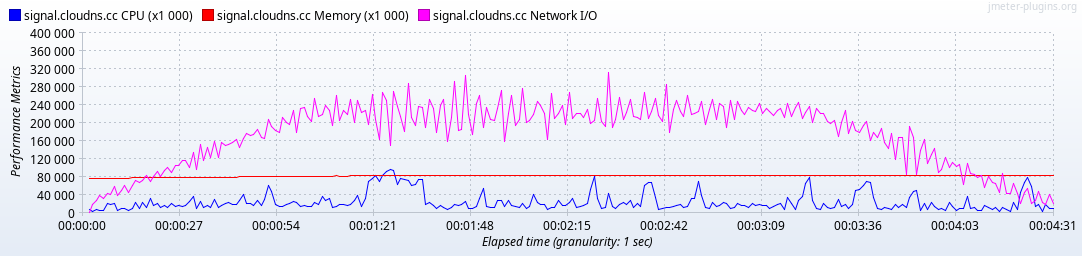
\includegraphics[width=\textwidth]{images/613/signal-create-load}
    \caption{High load accounts' creation on Signal 6.13}
    \label{fig:signalcreateloadnew}
\end{figure}



Here I report the results for the requests divided by type.

\begin{figure}[H]
    \centering
    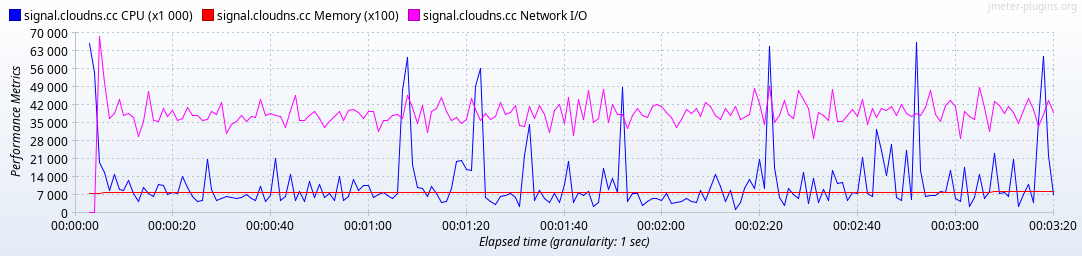
\includegraphics[width=\textwidth]{images/613/create-load-1}
    \caption{High load GET /v1/accounts/fcm/preauth on Signal 6.13}
    \label{fig:signalload1new}
\end{figure}

\begin{figure}[H]
    \centering
    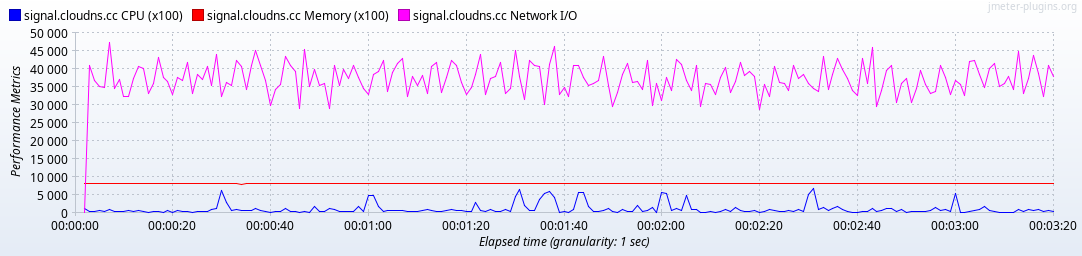
\includegraphics[width=\textwidth]{images/613/create-load-2}
    \caption{High load GET /v1/accounts/sms/code on Signal 6.13}
    \label{fig:signalload2new}
\end{figure}

\begin{figure}[H]
    \centering
    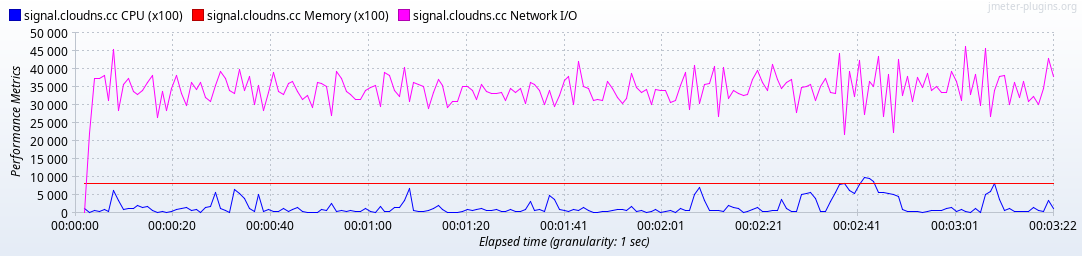
\includegraphics[width=\textwidth]{images/613/create-load-3}
    \caption{High load PUT /v1/accounts/code on Signal 6.13}
    \label{fig:signalload3new}
\end{figure}

\begin{figure}[H]
    \centering
    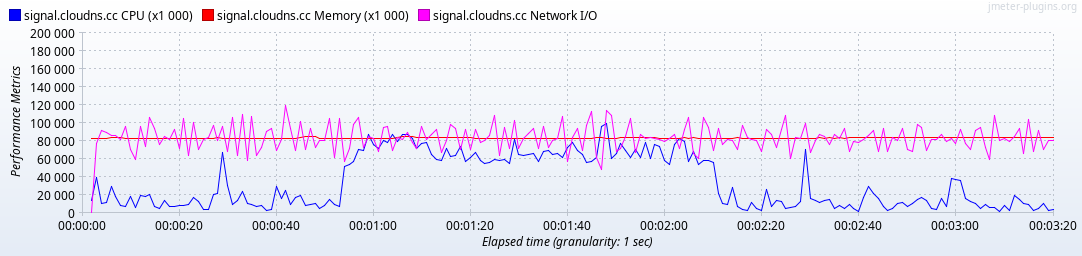
\includegraphics[width=\textwidth]{images/613/create-load-4}
    \caption{High load PUT /v2/keys on Signal 6.13}
    \label{fig:signalload4new}
\end{figure}

\begin{figure}[H]
    \centering
    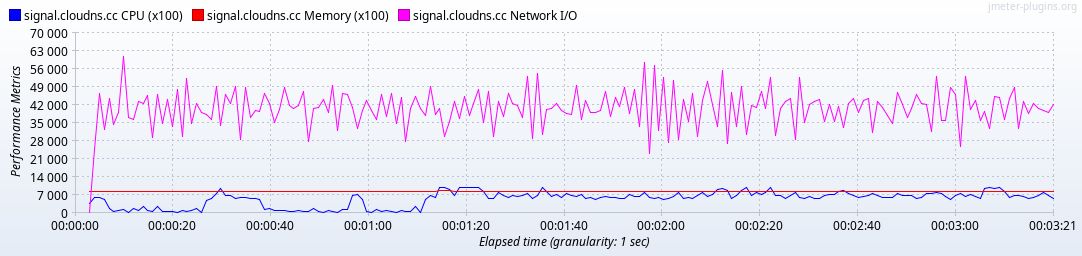
\includegraphics[width=\textwidth]{images/613/create-load-5}
    \caption{High load PUT /v1/accounts/gcm on Signal 6.13}
    \label{fig:signalload5new}
\end{figure}

\begin{figure}[H]
    \centering
    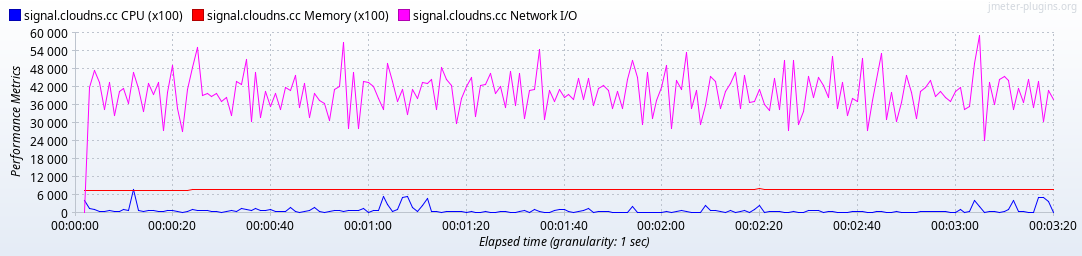
\includegraphics[width=\textwidth]{images/613/create-load-6}
    \caption{High load GET /v1/certificate/delivery on Signal 6.13}
    \label{fig:signalload6new}
\end{figure}

\begin{figure}[H]
    \centering
    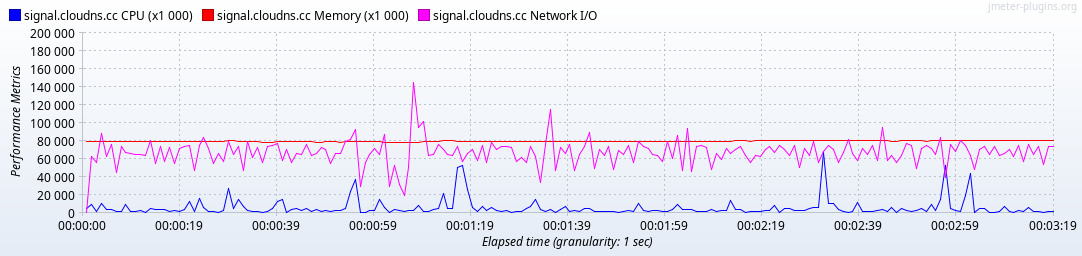
\includegraphics[width=\textwidth]{images/613/create-load-7}
    \caption{High load PUT /v1/directory/tokens on Signal 6.13}
    \label{fig:signalload7new}
\end{figure}

\begin{figure}[H]
    \centering
    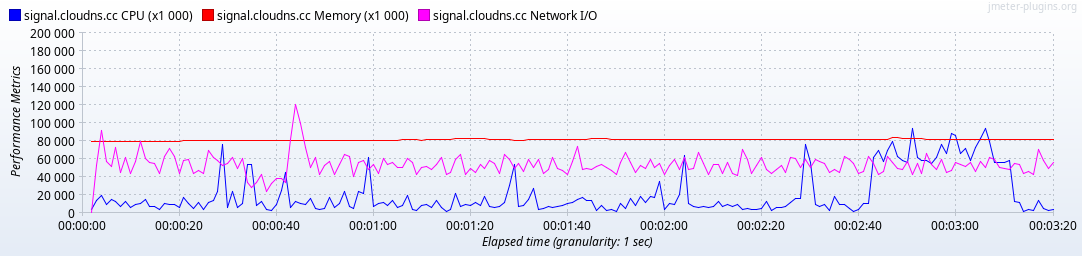
\includegraphics[width=\textwidth]{images/613/create-load-8}
    \caption{High load PUT /v1/profile on Signal 6.13}
    \label{fig:signalload8new}
\end{figure}

As on the 4.97 version, with the 6.13 version there are not overloads.

\subsection{New message sending\label{sec:newmessage}}

This experiment uses the following REST APIs:

\begin{table}[H]
\resizebox{\textwidth}{!}{%
\begin{tabular}{@{}llll@{}}
\hline
\multicolumn{1}{c}{\textbf{Type of request}} & \multicolumn{1}{c}{\textbf{Request path}} & \multicolumn{1}{c}{\textbf{Description}} & \multicolumn{1}{c}{\textbf{Involved components}} \\ \hline
GET & /v1/profile & Request data of the receiver profile & Dropwizard, Redis, PostgreSQL/DynamoDB \\
GET & /v2/keys/+390123456789/* & Get the keys for message encryption & Dropwizard, Redis, PostgreSQL/DynamoDB \\
PUT & /v1/messages & Send the message to the receiver & Dropwizard, Redis, PostgreSQL/DynamoDB \\\bottomrule
\end{tabular}%
}
\caption{Sequence of calls to send a message}
\label{tab:apimessage}
\end{table}

Between the request of the keys to send the message to the receiver and the request to send the message there is a think time of $3$ seconds, to simulate a low think time of the user when he writes the message.



\subsubsection{Base load for a long period of time on Signal 4.97}

Here I report the table with the results from the experiment on Signal 4.97.

\begin{table}[H]
\resizebox{\textwidth}{!}{%
\begin{tabular}{@{}lllllllllll@{}}
\hline
\multicolumn{1}{c}{\multirow{2}{*}{\textbf{Request}}} & \multicolumn{1}{c}{\multirow{2}{*}{\textbf{\#Samples}}} & \multicolumn{7}{c}{\textbf{Response times (ms)}} & \multicolumn{2}{c}{\textbf{Network (KB/s)}} \\ \cline{3-11} 
\multicolumn{1}{c}{} & \multicolumn{1}{c}{} & \multicolumn{1}{c}{Average} & \multicolumn{1}{c}{Min} & \multicolumn{1}{c}{Max} & \multicolumn{1}{c}{Median} & \multicolumn{1}{c}{90th pct} & \multicolumn{1}{c}{95th pct} & \multicolumn{1}{c}{99th pct} & \multicolumn{1}{c}{Received} & \multicolumn{1}{c}{Sent} \\ \hline
GET /v1/profile & 1000 & 56.68 & 33 & 308 & 53.00 & 78.00 & 87.95 & 112.99 & 0.48 & 0.32 \\
GET /v2/keys/+390123456789/* & 1000 & 26.73 & 19 & 306 & 24.00 & 33.00 & 42.00 & 57.00 & 0.33 & 0.09 \\
PUT /v1/messages & 1000 & 47.74 & 23 & 987 & 44.00 & 66.00 & 87.00 & 133.00 & 0.17 & 0.28 \\\bottomrule
\end{tabular}%
}
\caption{Base load message sending on Signal 4.97}
\label{tab:baseloadmessageold}
\end{table}

The request which requires more time for the response is the one used to obtain the receiver profile data.
This request uses more Redis and PostgreSQL if the data are not present on Redis.

Here I show the diagram with the resource use.

\begin{figure}[H]
    \centering
    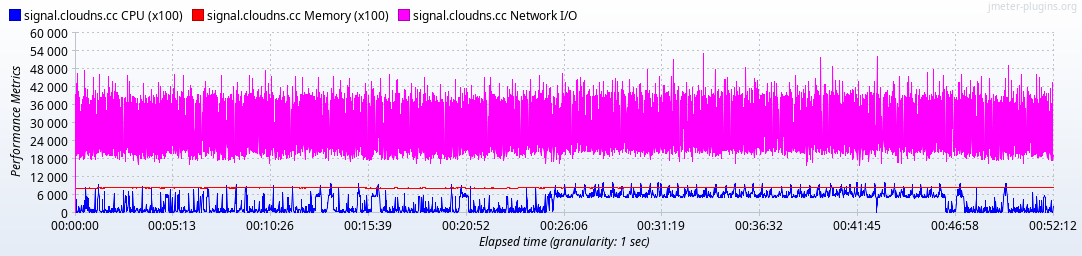
\includegraphics[width=\textwidth]{images/497/signal-base-message-load}
    \caption{Base load message sending on Signal 4.97}
    \label{fig:signalbasemessageloadold}
\end{figure}

From the diagram it is visible a higher load from the $26$th minute to the $46$th one, but there is no overload on the server.

\subsubsection{High load with ramp-up on Signal 4.97}

Here there are the data relative to the experiment with high load and ramp-up for sending messages.

\begin{table}[H]
\resizebox{\textwidth}{!}{%
\begin{tabular}{@{}lllllllllll@{}}
\hline
\multicolumn{1}{c}{\multirow{2}{*}{\textbf{Request}}} & \multicolumn{1}{c}{\multirow{2}{*}{\textbf{\#Samples}}} & \multicolumn{7}{c}{\textbf{Response times (ms)}} & \multicolumn{2}{c}{\textbf{Network (KB/s)}} \\ \cline{3-11} 
\multicolumn{1}{c}{} & \multicolumn{1}{c}{} & \multicolumn{1}{c}{Average} & \multicolumn{1}{c}{Min} & \multicolumn{1}{c}{Max} & \multicolumn{1}{c}{Median} & \multicolumn{1}{c}{90th pct} & \multicolumn{1}{c}{95th pct} & \multicolumn{1}{c}{99th pct} & \multicolumn{1}{c}{Received} & \multicolumn{1}{c}{Sent} \\ \hline
GET /v1/profile & 1000 & 174.16 & 31 & 130122 & 37.00 & 80.00 & 91.00 & 114.00 & 5.68 & 3.78 \\
GET /v2/keys/+390123456789/* & 1000 & 25.19 & 19 & 306 & 24.00 & 27.00 & 33.00 & 54.99 & 3.89 & 1.04 \\
PUT /v1/messages & 1000 & 26.55 & 22 & 97 & 25.00 & 29.00 & 35.00 & 52.98 & 2.00 & 3.26 \\\bottomrule
\end{tabular}%
}
\caption{High load message sending on Signal 4.97}
\label{tab:highloadmessageold}
\end{table}

In this case, as on the previous one, the order of the requests is the same for the response time.
The following diagram shows the resources use.

\begin{figure}[H]
    \centering
    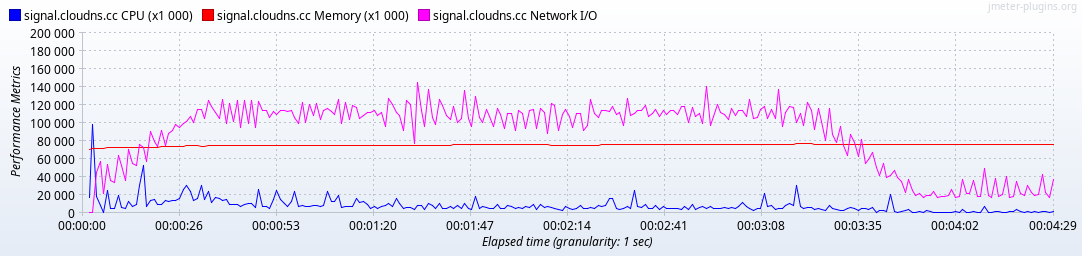
\includegraphics[width=\textwidth]{images/497/signal-message-load}
    \caption{High load message sending on Signal 4.97}
    \label{fig:signalmessageloadold}
\end{figure}

The diagram confirms the scale-up, so the requests are queued, but there is no overload on the server for the CPU usage.

To verify which requests require more resources, I did the same experiment as before, looking on the single type requests.


\begin{figure}[H]
    \centering
    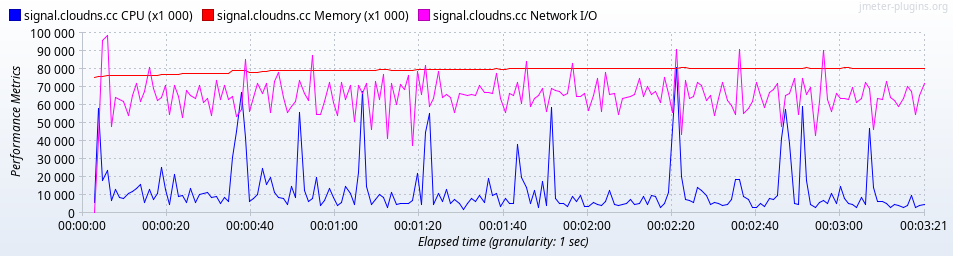
\includegraphics[width=\textwidth]{images/497/message-load-1}
    \caption{High load GET /v1/profile on Signal 4.97}
    \label{fig:signalload1oldmessage}
\end{figure}


\begin{figure}[H]
    \centering
    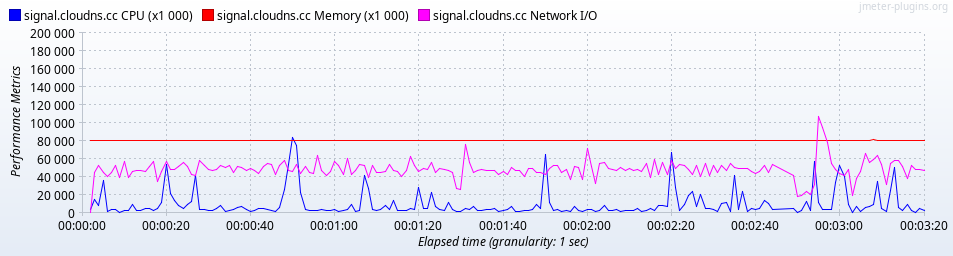
\includegraphics[width=\textwidth]{images/497/message-load-2}
    \caption{High load GET /v2/keys/+390123456789/* on Signal 4.97}
    \label{fig:signalload2oldmessage}
\end{figure}


\begin{figure}[H]
    \centering
    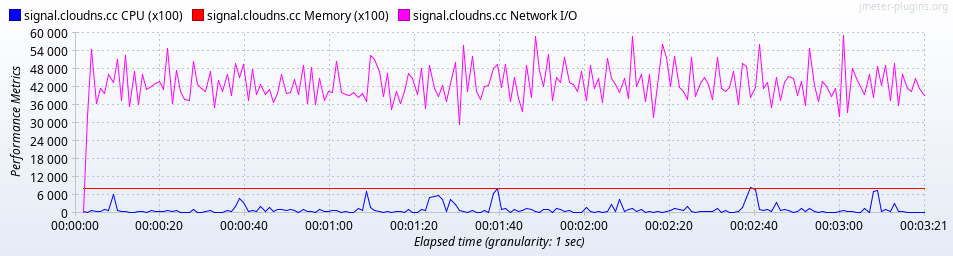
\includegraphics[width=\textwidth]{images/497/message-load-3}
    \caption{High load PUT /v1/messages on Signal 4.97}
    \label{fig:signalload3oldmessage}
\end{figure}

In this case all the three kind of request finish in a correct way, without overloads.

Here I compare the previous results with the 6.13 Signal server version.

\subsubsection{Base load for a long period of time on Signal 6.13}

The following table has got the measures for the message sending on Signal 6.13.

\begin{table}[H]
\resizebox{\textwidth}{!}{%
\begin{tabular}{@{}lllllllllll@{}}
\hline
\multicolumn{1}{c}{\multirow{2}{*}{\textbf{Request}}} & \multicolumn{1}{c}{\multirow{2}{*}{\textbf{\#Samples}}} & \multicolumn{7}{c}{\textbf{Response times (ms)}} & \multicolumn{2}{c}{\textbf{Network (KB/s)}} \\ \cline{3-11} 
\multicolumn{1}{c}{} & \multicolumn{1}{c}{} & \multicolumn{1}{c}{Average} & \multicolumn{1}{c}{Min} & \multicolumn{1}{c}{Max} & \multicolumn{1}{c}{Median} & \multicolumn{1}{c}{90th pct} & \multicolumn{1}{c}{95th pct} & \multicolumn{1}{c}{99th pct} & \multicolumn{1}{c}{Received} & \multicolumn{1}{c}{Sent} \\ \hline
GET /v1/profile & 1000 & 56.68 & 33 & 308 & 53.00 & 78.00 & 87.95 & 112.99 & 0.48 & 0.32 \\
GET /v2/keys/+390123456789/* & 1000 & 26.73 & 19 & 306 & 24.00 & 33.00 & 42.00 & 57.00 & 0.33 & 0.09 \\
PUT /v1/messages & 1000 & 47.74 & 23 & 987 & 44.00 & 66.00 & 87.00 & 133.00 & 0.17 & 0.28 \\\bottomrule
\end{tabular}%
}
\caption{Base load message sending on Signal 6.13}
\label{tab:baseloadmessagenew}
\end{table}

As for the 4.97 version of the server, the requests to get the profile data of the receiver and to send the messages are the ones which needs a higher response time, but their distance is higher this time.

The following diagram shows the resource usage.

\begin{figure}[H]
    \centering
    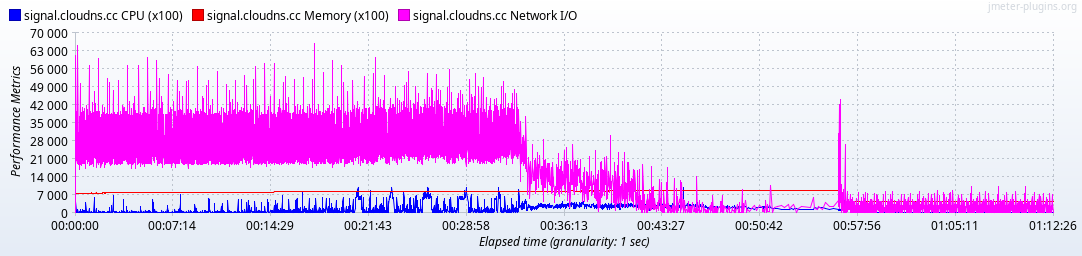
\includegraphics[width=\textwidth]{images/613/signal-base-message-load}
    \caption{Base load message sending on Signal 6.13}
    \label{fig:signalbasemessageloadnew}
\end{figure}

Compared to the 4.97 version of the server, there is a rejection of requests after $30$ minutes from the starting point of the experiment, this is the reason of the traffic decrease.
As a consequence the CPU use decreases.

On the next section there are the high load results.

\subsubsection{High load with ramp-up on Signal 6.13}

Here the data relative to the high load with ramp-up period.

\begin{table}[H]
\resizebox{\textwidth}{!}{%
\begin{tabular}{@{}lllllllllll@{}}
\toprule
\multicolumn{1}{c}{\multirow{2}{*}{\textbf{Request}}} & \multicolumn{1}{c}{\multirow{2}{*}{\textbf{\#Samples}}} & \multicolumn{7}{c}{\textbf{Response times (ms)}} & \multicolumn{2}{c}{\textbf{Network (KB/s)}} \\ \cmidrule(l){3-11} 
\multicolumn{1}{c}{} & \multicolumn{1}{c}{} & \multicolumn{1}{c}{Average} & \multicolumn{1}{c}{Min} & \multicolumn{1}{c}{Max} & \multicolumn{1}{c}{Median} & \multicolumn{1}{c}{90th pct} & \multicolumn{1}{c}{95th pct} & \multicolumn{1}{c}{99th pct} & \multicolumn{1}{c}{Received} & \multicolumn{1}{c}{Sent} \\ \midrule
GET /v1/profile & 1000 & 54.95 & 34 & 328 & 43.00 & 98.00 & 112.00 & 152.98 & 7.02 & 4.45 \\
GET /v2/keys/+390123456789/* & 1000 & 27.91 & 20 & 495 & 24.00 & 37.00 & 46.95 & 64.97 & 4.35 & 1.22 \\
PUT /v1/messages & 1000 & 28.89 & 22 & 123 & 26.00 & 37.00 & 43.00 & 59.99 & 2.35 & 3.84 \\ \bottomrule
\end{tabular}%
}
\caption{High load message sending on Signal 6.13}
\label{tab:highloadmessagenew}
\end{table}

Here the median response times are comparable to the 4.97 version.
The load is higher compared to the other version, but there is no overload.
It is clearly visible the ramp-up on the following diagram.

\begin{figure}[H]
    \centering
    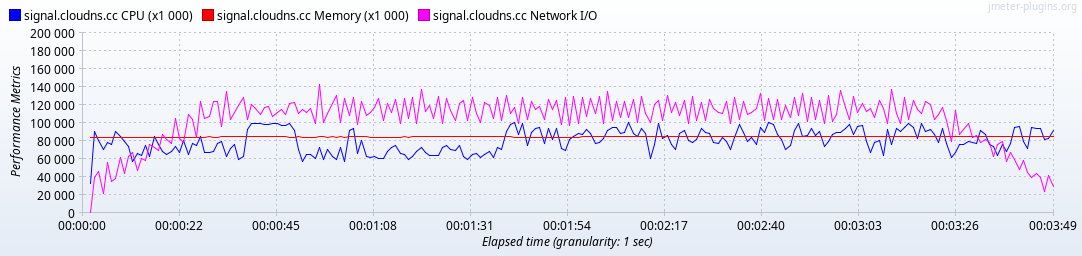
\includegraphics[width=\textwidth]{images/613/signal-message-load}
    \caption{High load message sending on Signal 6.13}
    \label{fig:signalhighmessageloadnew}
\end{figure}

The following diagrams report the resource usage for the requests divided by type.

\begin{figure}[H]
    \centering
    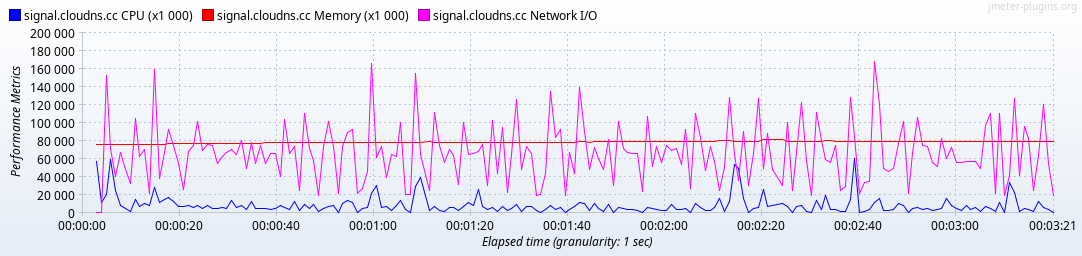
\includegraphics[width=\textwidth]{images/613/message-load-1}
    \caption{High load GET /v1/profile on Signal 6.13}
    \label{fig:signalload1newmessage}
\end{figure}


\begin{figure}[H]
    \centering
    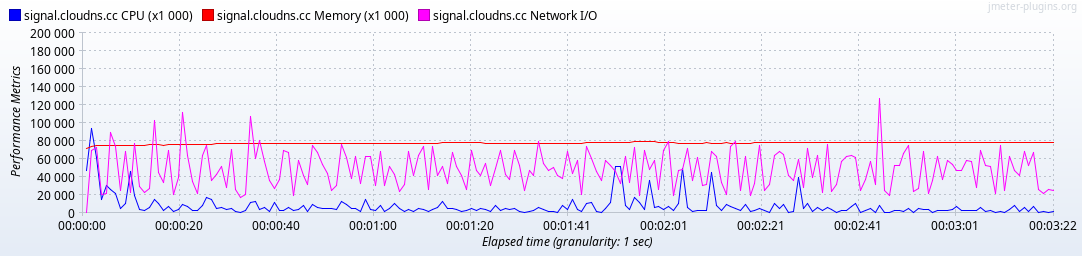
\includegraphics[width=\textwidth]{images/613/message-load-2}
    \caption{High load GET /v2/keys/+390123456789/* on Signal 6.13}
    \label{fig:signalload2newmessage}
\end{figure}


\begin{figure}[H]
    \centering
    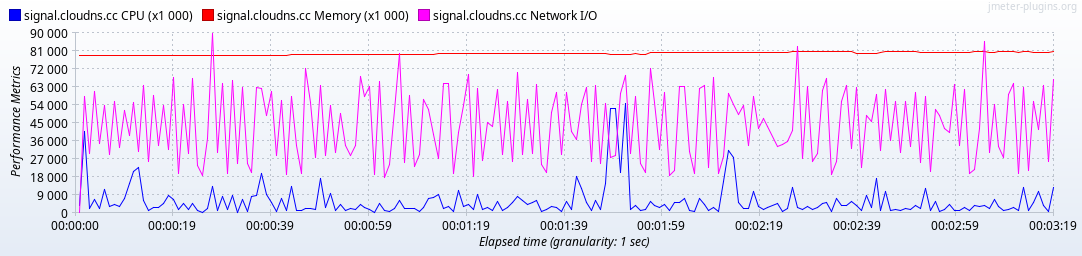
\includegraphics[width=\textwidth]{images/613/message-load-3}
    \caption{High load PUT /v1/messages on Signal 6.13}
    \label{fig:signalload3newmessage}
\end{figure}

As in the previous experiments, there is no overload, only some queued requests between the minute $1:40$ and the minute $1:50$.

\section{Observations\label{sec:observations}}

From the performed experiments there are no evidence about a load due to the single API calls.
What can be deducted is that while the first architecture model, which uses PostgreSQL and less AWS services, reacts better to less intensive loads for long periods of time, while the second model, which uses DynamoDB and other AWS services not present before, reacts better to more intensive loads and more concentrated in a short period of time.

It is reasonable saying that the outage happened on January 2021 as described on the Signal community blog \cite{outage} happened because of an accumulation of sessions made from the Android clients in order to retry the failed message sending, without success, and making the situation worse.

The given solution was on the client side, to automatically reset the connection, so they released the resources from the server, which were necessary to manage the new incoming connections.